%% Numbers checked against artifact_fmcg_abc.json (first iteration), artifact_fmcg_abc_v2.json (second iteration), generated/tab_decomp.tex, tab_artifact.tex, tab_resources.tex.
This section demonstrates the decision artifact on the median FMCG-ABC policy of the main instance. The artifact is produced by the same code that the DSS service calls; in the DSS the replay-based fields are only available when a holdout replay has been run, and the rules that need them (R1, R6) are then reported as not evaluated rather than silently omitted.

\subsection{Economic explanation}
Table~\ref{tab:decomp} decomposes the model cost. Compared with the (infeasible) EOQ policy, the feasible FMCG-ABC policy orders smaller quantities for 33 of the 50 SKUs, which raises ordering cost by 82\% and lowers holding cost by 13\%; it takes the quantity discount for 17 SKUs, and purchasing cost rises by 1.3\% because the budget no longer allows the discount to be taken for every SKU where it pays. Total model cost is 1.4\% higher than the EOQ cost. Because the EOQ policy violates both limits, this is not a comparison of two admissible policies: it measures how much the unconstrained economic optimum understates the cost of a policy the organisation can actually finance and store (on the controllable scale, 16.0 against 34.1 million). At SKU level, holding is the largest controllable cost component for 30 SKUs and ordering for 20; shortage is never the largest. A manager therefore sees immediately that the policy is shaped by the trade-off between order frequency and stock investment under binding resources, not by shortage risk.

\begin{table}[!htbp]
\centering
\footnotesize
\caption{Model cost decomposition (millions per year): EOQ with static safety stock versus the median FMCG-ABC policy on the main instance.}\label{tab:decomp}
\begin{tabular}{lrrr}
\toprule
Component & EOQ + static SS & FMCG-ABC & Change (\%) \\
\midrule
Ordering & 2.93 & 5.32 & +81.5 \\
Holding & 11.37 & 9.94 & -12.5 \\
Shortage & 1.67 & 1.71 & +2.4 \\
Purchasing & 1,310.65 & 1,327.77 & +1.3 \\
Total & 1,326.62 & 1,344.75 & +1.4 \\
\bottomrule
\end{tabular}
\par\smallskip\parbox{0.95\linewidth}{\scriptsize The EOQ policy violates the coupling constraints (budget utilisation 133\%); FMCG-ABC budget utilisation 99.9\%, warehouse utilisation 95.2\%, 99.8\%.}
\end{table}


\subsection{Constraint and service explanation}
The policy uses 99.9\% of the budget and 95.2\% and 99.8\% of the two warehouses. Utilisation alone does not say which limits constrain the policy: the budget and the second warehouse are at their limits and have positive multipliers in the bound, whereas the first warehouse is highly used but its multiplier is zero (Table~\ref{tab:resources}). In the model, every SKU meets its service target, 15 of them exactly at the bound $SS_i=z_{\alpha_i}\sigma_{DLT,i}$. In the replay, 27 SKUs fall short of their target, the portfolio cycle service level is 92.9\% and the fill rate 99.3\%. The expected shortage exposure $ESE_i=ES_i/Q_i$ has a median of 0.31\% and a maximum of 1.8\% of annual demand.

\subsection{Recommendations and an SKU record}
Table~\ref{tab:rules} lists the recommendation rules. Their thresholds were fixed before the experiments and are stored with every artifact. Rules R1--R3 and R6 describe an SKU; R4 and R5 describe a shared resource and, after the first evaluation (below), are reported once per resource rather than in each SKU record.

\begin{table}[!htbp]
\centering\footnotesize
\caption{Recommendation rules (condition $\to$ evidence $\to$ action).}\label{tab:rules}
\begin{tabular}{@{}ll>{\raggedright\arraybackslash}p{0.3\linewidth}>{\raggedright\arraybackslash}p{0.15\linewidth}>{\raggedright\arraybackslash}p{0.27\linewidth}@{}}
\toprule
ID & Scope & Condition & Evidence & Action \\
\midrule
R1 & SKU & $CV_{d,i}>0.50$ and realised CSL $<\alpha_i$ & $CV$, realised CSL & increase protection, subject to budget and capacity \\
R2 & SKU & holding share of controllable cost $>0.50$ & $C_{h,i}/\Cctrl_i$ & review / reduce order quantity \\
R3 & SKU & $L_i>14$ days & $L_i$ & review supplier lead-time arrangement \\
R4 & resource & $U_w>0.95$; status from limit and multiplier $\mu_w$ & $U_w$, $\mu_w$ & redistribute or reduce inventory exposure \\
R5 & resource & $U_B>0.95$; status from limit and multiplier $\lambda$ & $U_B$, $\lambda$ & delay, split or reprioritise procurement \\
R6 & SKU & realised CSL $<\alpha_i-0.05$ and $ESE_i>0.01$ & CSL, $ESE_i$ & prioritise service protection \\
\bottomrule
\end{tabular}
\end{table}
 In the first design iteration, evaluated here, every rule was attached to SKU records, and on this policy the rules fired 155 times: R4 (warehouse) and R5 (budget) for all 50 SKUs, R2 (holding-dominated cost) for 27, R3 (long lead time) for 16, R1 (high variability with realised service below target) for 12, and R6 never. R4 and R5 carried no SKU-specific information, and R4 fired for every SKU of the first warehouse although that warehouse does not constrain the policy (see below). In the second iteration, which the DSS now implements, the SKU records contain only R1--R3 and R6 (55 firings on this policy), and the resources are reported once (Table~\ref{tab:resources}) with one of four statuses: \emph{constraining} (at the limit, utilisation $\ge99.5\%$, with a positive multiplier), \emph{high utilisation, not constraining} (above the threshold with a zero multiplier), \emph{high utilisation, marginal value not computed} (when no bound was computed), and \emph{not constraining}. Table~\ref{tab:artifact} shows the record of the SKU with the most rules fired. Its order quantity exceeds the EOQ (1{,}496 vs.\ 943 units) because ordering at least the discount threshold earns the lower price; holding is 85\% of its controllable cost, its lead time is 20 days, its demand is highly variable ($CV=0.70$), and its realised service (0.949) is below its target (0.98) although the model-implied value meets it. The record states each of these facts with the number behind it and the action it suggests, and leaves the trade-off between them to the manager: R1 suggests more protection, R2 a smaller order quantity, and the resource view adds that this SKU's warehouse is highly used but not constraining, whereas the budget is constraining, so additional protection must be financed by savings elsewhere in the portfolio.

\begin{table}[!htbp]
\centering
\footnotesize
\caption{SKU-level decision artifact generated by the system for one SKU of the main instance (median FMCG-ABC run). Every entry is computed from the policy, the model or the replay.}\label{tab:artifact}
\begin{tabular}{p{0.38\linewidth}p{0.55\linewidth}}
\toprule
Field & Value \\
\midrule
SKU & SIM-040 (warehouse 0) \\
Order quantity $Q_i$ (EOQ baseline) & 1,496 (943) \\
Safety stock $SS_i$ (baseline) & 1,030 (1,030) \\
Reorder point $ROP_i$ & 2,952 \\
Price paid / discount taken & 1,385.45 / yes \\
Ordering / holding / shortage cost & 51,947 / 723,971 / 73,236 \\
Purchasing cost & 48,606,996 \\
Primary controllable driver & holding (85\%) \\
Model / target / realised CSL & 0.980 / 0.98 / 0.949 \\
Realised fill rate & 0.9887 \\
Budget / warehouse utilisation & 99.9\% / 95.2\% \\
Rule R1 & CV 0.70 $>$ 0.5 and realised CSL 0.949 $<$ target 0.98 $\Rightarrow$ Increase protection inventory, subject to budget and warehouse capacity \\
Rule R2 & holding cost is 85\% of controllable cost $\Rightarrow$ Review / reduce the order quantity \\
Rule R3 & lead time 20 d $>$ 14 d $\Rightarrow$ Review the supplier lead-time arrangement \\
\bottomrule
\end{tabular}
\end{table}


\begin{table}[!htbp]
\centering
\footnotesize
\caption{Portfolio-level resource view of the median FMCG-ABC policy (second design iteration): utilisation, whether the limit is reached, and the multiplier of the Lagrangian bound.}\label{tab:resources}
\resizebox{\linewidth}{!}{%
\begin{tabular}{>{\raggedright\arraybackslash}p{0.17\linewidth}lrrr>{\raggedright\arraybackslash}p{0.17\linewidth}>{\raggedright\arraybackslash}p{0.42\linewidth}}
\toprule
Resource & Rule & Use (\%) & At limit & Multiplier & Status & Action \\
\midrule
Procurement budget & R5 & 99.9 & yes & 0.91 & constraining & Relieving this resource lowers cost; compare the marginal value with its price before requesting more. \\
Warehouse 0 & R4 & 95.2 & no & 0.00 & high use, not constraining & Monitor; at the current policy the limit does not raise cost. \\
Warehouse 1 & R4 & 99.8 & yes & 17,924.42 & constraining & Relieving this resource lowers cost; compare the marginal value with its price before requesting more space. \\
\bottomrule
\end{tabular}}
\par\smallskip\parbox{0.95\linewidth}{\scriptsize At limit: utilisation of at least 99.5\%. Multipliers from the best dual point of the E1 bound (budget: per currency unit; warehouses: per m$^3$); with quantity discounts they are sensitivities of the bound, not exact shadow prices of the optimal cost.}
\end{table}


\subsection{Fidelity and an observation for redesign}
By construction, every number in the artifact is recomputed from $(Q,SS)$ with the model of Section~\ref{sec:model} or taken from the replay, and the automated tests check that the cost components sum to the reported total and that each fired rule's evidence satisfies its condition (for example, that R3 fires only for lead times above the threshold). This gives explanation fidelity in the sense of a traceable recommendation $\to$ evidence $\to$ model-output chain; it does not establish that the explanations improve managers' decisions, which requires a user study. As an example of the chain, the R2 entry of Table~\ref{tab:artifact} traces to the holding cost $h_i(Q_i/2+SS_i)=723{,}971$ and the controllable cost $51{,}947+723{,}971+73{,}236=849{,}154$ of the same SKU, whose ratio 0.85 exceeds the threshold 0.50; a test recomputes this chain.

The artifact provides three kinds of explanation, and we claim no more for it. (i) \emph{Descriptive} explanations decompose the model cost of the recommended policy into its components and report utilisation and service (Tables~\ref{tab:decomp} and \ref{tab:artifact}). (ii) \emph{Model-based diagnostics} compare these quantities with thresholds fixed in advance (the rules) or with the dual information of the bound (the resource status). (iii) \emph{Counterfactual sensitivity} is obtained by re-optimising or recomputing the bound under a changed resource (Tables~\ref{tab:s2} and \ref{tab:sens}). None of them is causal: a rule states that a condition holds for the recommended policy, not that acting on it will improve the outcome, and the cost decomposition is an accounting identity of the model, not an attribution of realised costs.

The evaluation exposed a weakness of the first rule design, which led to the second iteration described above. Because an optimised policy exhausts the binding resources, the threshold rules R4 and R5 fire for every SKU in the warehouse or portfolio and carry no SKU-specific information, and high utilisation is not the same as a binding limit, nor a binding limit the same as a positive marginal value. The resources are therefore reported once at portfolio level, together with the value of relieving them, which the bound already provides. At the dual solution of the main instance, the budget multiplier is $\lambda=0.91$ and the warehouse multipliers are $\mu=(0,\;17{,}924)$ per m$^3$: the second warehouse binds in the relaxation, the first does not. Their first-order estimate for a 10\% change of the budget ($\pm3.73$ million) is close to the recomputed change of the bound ($+3.91$ million for a 10\% cut, $-3.22$ million for a 10\% increase; S2, Table~\ref{tab:s2}); for the capacities the response is asymmetric ($+1.23$ and $-0.12$ million against an estimate of $\pm0.49$ million), because the multipliers change once the second warehouse is relieved. These are changes of a lower bound, not of the cost of a particular policy, and with discounts the multipliers are only approximate shadow prices; they are nevertheless the kind of evidence a planner needs to decide whether to request more budget or space. The re-optimised FMCG-ABC policies move in the same direction (Table~\ref{tab:sens}).

\begin{table}[!htbp]
\centering\footnotesize
\caption{Change of the Lagrangian lower bound of the main instance when a resource is scaled (S2), against the first-order estimate from the multipliers (millions).}\label{tab:s2}
\begin{tabular}{lrrr}
\toprule
Scenario & Bound (controllable) & Change of bound & First-order estimate \\
\midrule
Base & 25.02 & -- & -- \\
$B\times0.9$ & 28.93 & $+3.91$ & $+3.73$ \\
$B\times1.1$ & 21.80 & $-3.22$ & $-3.73$ \\
$Cap_w\times0.9$ & 26.25 & $+1.23$ & $+0.49$ \\
$Cap_w\times1.1$ & 24.90 & $-0.12$ & $-0.49$ \\
\bottomrule
\end{tabular}
\end{table}

\subsection{The artifact in the decision support system}
Figure~\ref{fig:iid} shows the same artifact as the IID presents it, computed on the synthetic sample file distributed with the system (64 SKUs, no discount data, so the bound certifies the gap; values are illustrative and unrelated to the study instance). The planner selects a method and obtains the feasibility status, model cost, lower bound and certified gap (2.5\% here), budget and warehouse utilisation, the EOQ baseline, the count of fired rules with the rules that could not be evaluated without a replay, and one row per SKU with its policy, cost components, primary cost driver, model-implied service and the evidence and action of each fired rule; the mapping from inventory records to model parameters is stated below the table. Following the evaluation above, a second design iteration of the IID view reports binding resources once at portfolio level, with their shadow prices and the first-order saving from 10\% more of each resource; because the dashboard records hold no discount data, the model is convex there, the bound is tight, and the multipliers are the shadow prices of the optimal cost (where it is differentiable). Figure~\ref{fig:iid} shows why this matters: under the first rule design R5 would fire for all 64 SKUs because the policy uses 96.4\% of the budget, but the shadow price of the budget is zero, so the budget does not in fact constrain the policy; the view reports it as ``high utilisation, not constraining'' and every warehouse pool as not constraining. Recommendations are then accepted, modified or rejected in the decision workflow of Section~\ref{sec:framework}.

\begin{figure}[!htbp]
\centering
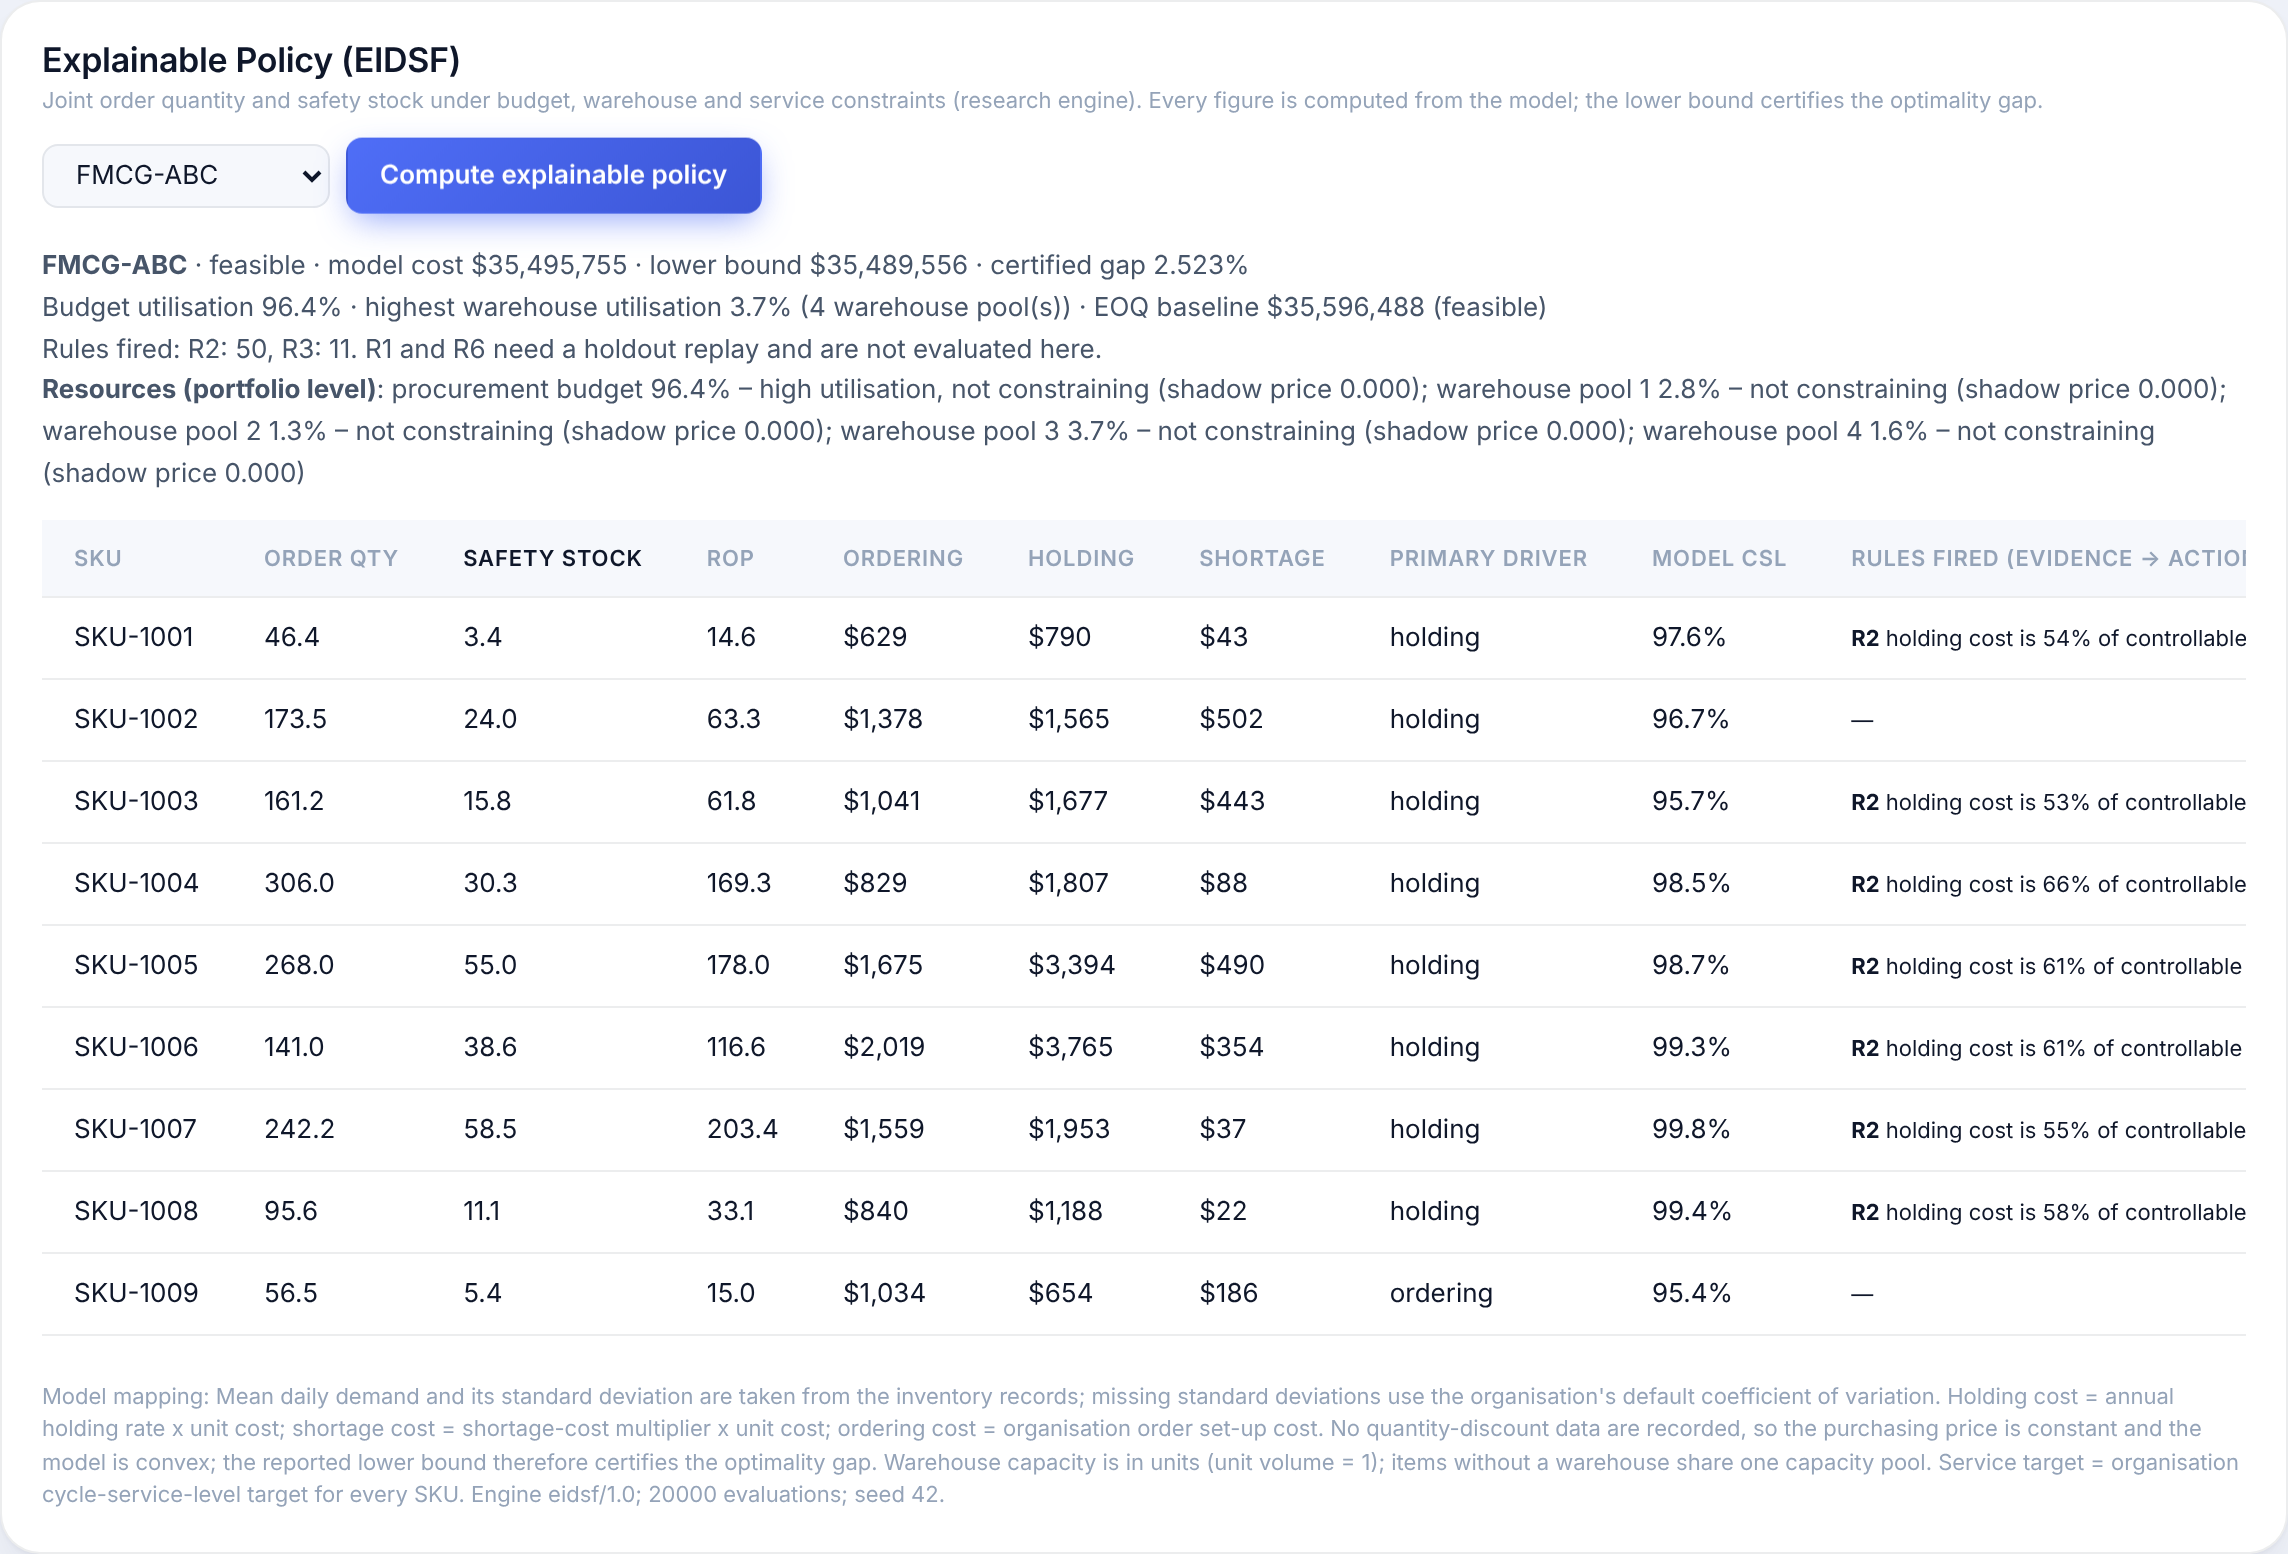
\includegraphics[width=\linewidth]{figures/fig_dashboard.png}
\caption{The explainable-policy view of the Inventory Intelligence Dashboard (FMCG-ABC, seed 42, 20{,}000 evaluations) on the synthetic sample file shipped with the system, after the second design iteration (portfolio-level resource status). The certified gap refers to the controllable cost. The rules column is truncated in the screenshot.}\label{fig:iid}
\end{figure}
